\begin{figure}[H]
    \centering
    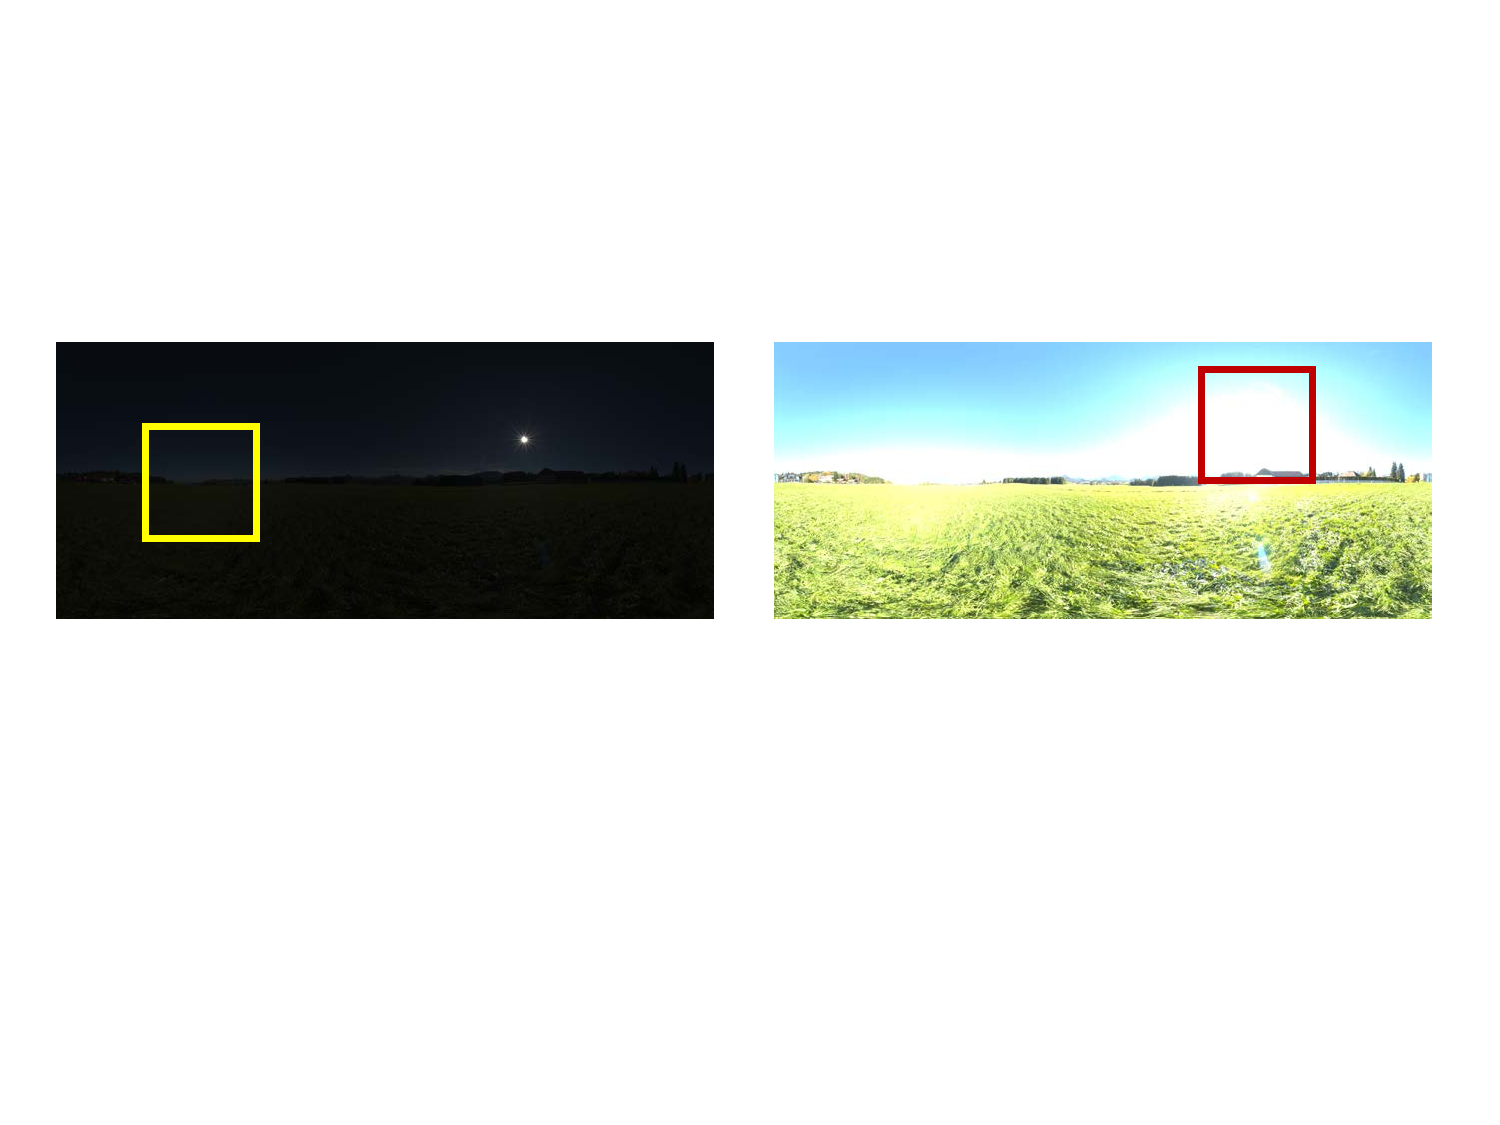
\includegraphics[width=1.0\textwidth]{Img/different-exposure.pdf}
    \caption[使用不同曝光拍摄的LDR图像]
    {两种不同曝光条件下的LDR图像。在欠曝图像中,黄色框选区域中大部分像素均为黑色,但它们的明暗程度并不同;类似地,在过曝图像中,红色框选区域中像素值均为白色,但实际上太阳所处像素的亮度远远高于周围像素。使用LDR图像难以解决这些问题。}
    \label{fig:different-exposure}
\end{figure}